% Name: Binary heap and its array
% Description: A min-heap drawn as a tree, with the same keys in the array that stores it.
% Tags: heap, priority queue, array, data structure

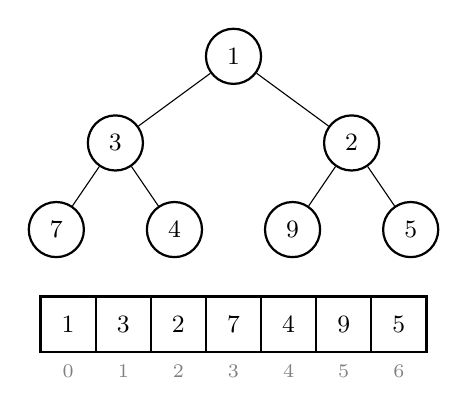
\begin{tikzpicture}[
  level distance=11mm,
  level 1/.style={sibling distance=30mm},
  level 2/.style={sibling distance=15mm},
  key/.style={circle, draw, thick, minimum size=7mm, inner sep=0pt, font=\small},
  cell/.style={draw, thick, minimum size=7mm, font=\small},
]
  \node[key] {1}
    child { node[key] {3}
      child { node[key] {7} }
      child { node[key] {4} }
    }
    child { node[key] {2}
      child { node[key] {9} }
      child { node[key] {5} }
    };
  \foreach \k [count=\i from 0] in {1, 3, 2, 7, 4, 9, 5} {
    \node[cell] at (\i*0.7 - 2.1, -3.4) {\k};
    \node[font=\scriptsize, gray] at (\i*0.7 - 2.1, -4) {\i};
  }
\end{tikzpicture}
